\section{Empirical evidence: identification and decision dynamics}
\label{sec:experiments}

We evaluate factor recovery in trained modules attached to pretrained
language models, varying the observation noise and query design. We then
test whether the recovered coordinates improve a structural decision.
These experiments measure numerical behavior on selected factorizations;
the global guarantees and their constants come from the theory. Earlier synthetic and byte-LM studies,
including large errors and failed rejection rules, remain in
Appendix~\ref{app:earlier-illustrations}.

\subsection{Factor recovery across pretrained models}

\paragraph{Nine models, a fixed module, and held-out gradient domains.}
We use three Pythia sizes (160M, 1B, 2.8B), four dense Qwen3 sizes
(0.6B, 1.7B, 4B, 8B), and two SmolLM2 sizes (360M, 1.7B)
\citep{biderman2023pythia,yang2025qwen3,allal2025smollm2}.
Each frozen BF16 backbone receives a $K=4$ softmax-shared additive module
on 64 fixed output channels of every attention output projection. Its bases
are direct trainable matrices, not LoRA products. A fixed isometric
embedding preserves the factor-response model
(Proposition~\ref{prop:llm-embedding}). We train only these modules for
256 AdamW updates on WikiText-2, using three seeds per model and the final
checkpoint. The resulting 27 checkpoints share nine fixed pretrained backbones, with
three adapter-training replicates per backbone.

Natural queries are measured next-token-loss gradients from disjoint
 general-text, MBPP code, and GSM8K math documents
\citep{merity2016wikitext,austin2021mbpp,cobbe2021gsm8k}.
The code and math domains are not used for adaptation or calibration.
Responses are controlled reverse-gradient/forward-JVP observations of the
factor map in FP64, treating the measured BF16-backbone gradients as fixed
inputs. These measurements require internal access to the product and
matrix-valued responses. They measure the controlled Euclidean response,
rather than the AdamW updates used to train the adapters.
The full protocol, model revisions, rejected access requests, development
corrections, and data/source hashes are in Appendix~\ref{app:llm-study}.

\paragraph{Finite recovery across model sizes and query types.}
We compare the repeated-complement design of
Corollary~\ref{cor:finite-noisy-main}, Gaussian queries, and three natural
 gradient families, with $q\in\{1,4,8\}$, four independent held-out
 directions, and relative noise $0,10^{-6},10^{-4},10^{-2}$ added to both
product and responses. The noisy product subspace is re-estimated and
orthogonal residuals are retained. Three estimators use observations only;
permutation-aligned ground truth is supplied afterward for scoring.

All 1,080 cases with $q\ge4$ met the observed rank conditions. Joint-fit
factor error was below $0.034$ in every case, with median
$1.86\times10^{-5}$. At $q=4$ without noise, the worst error across all
models and query families is $8.31\times10^{-13}$.
Table~\ref{tab:llm-models} reports maxima rather than selected seeds.
All 540 cases with $q=1$ failed the sufficient local-rank check and were
rejected before joint fitting. This failure concerns the specified
reconstruction condition; it leaves open what other one-query estimators
could recover.

\begin{table}[t]
\centering\small
\caption{Joint-fit factor error with $q=4$: maxima over three adaptation seeds, and (for natural queries) three text domains. Noise affects both product and response. $D$ is the adapter basis dimension, not the backbone parameter count. Each reported maximum includes all declared cases.}
\label{tab:llm-models}
\begin{tabular}{lrrrrr}
\toprule
Model & $L$ & $D$ & Natural, $0$ & Natural, $10^{-4}$ & Designed, $10^{-4}$\\
\midrule
Pythia 160M & 12 & 49152 & $6.5\!\times\!10^{-14}$ & $1.6\!\times\!10^{-4}$ & $1.4\!\times\!10^{-4}$\\
Pythia 1B & 16 & 131072 & $2.8\!\times\!10^{-13}$ & $5.7\!\times\!10^{-5}$ & $5.7\!\times\!10^{-5}$\\
Pythia 2.8B & 32 & 163840 & $8.3\!\times\!10^{-13}$ & $3.9\!\times\!10^{-5}$ & $3.8\!\times\!10^{-5}$\\
Qwen3 0.6B & 28 & 131072 & $6.6\!\times\!10^{-14}$ & $4.9\!\times\!10^{-5}$ & $4.9\!\times\!10^{-5}$\\
Qwen3 1.7B & 28 & 131072 & $9.2\!\times\!10^{-14}$ & $4.2\!\times\!10^{-5}$ & $4.2\!\times\!10^{-5}$\\
Qwen3 4B & 36 & 262144 & $1.0\!\times\!10^{-13}$ & $3.7\!\times\!10^{-5}$ & $3.7\!\times\!10^{-5}$\\
Qwen3 8B & 36 & 262144 & $2.6\!\times\!10^{-13}$ & $3.7\!\times\!10^{-5}$ & $3.6\!\times\!10^{-5}$\\
SmolLM2 360M & 32 & 61440 & $7.8\!\times\!10^{-14}$ & $3.8\!\times\!10^{-5}$ & $3.8\!\times\!10^{-5}$\\
SmolLM2 1.7B & 24 & 131072 & $6.4\!\times\!10^{-14}$ & $4.5\!\times\!10^{-5}$ & $4.4\!\times\!10^{-5}$\\
\bottomrule
\end{tabular}
\end{table}


\begin{figure}[t]
\centering
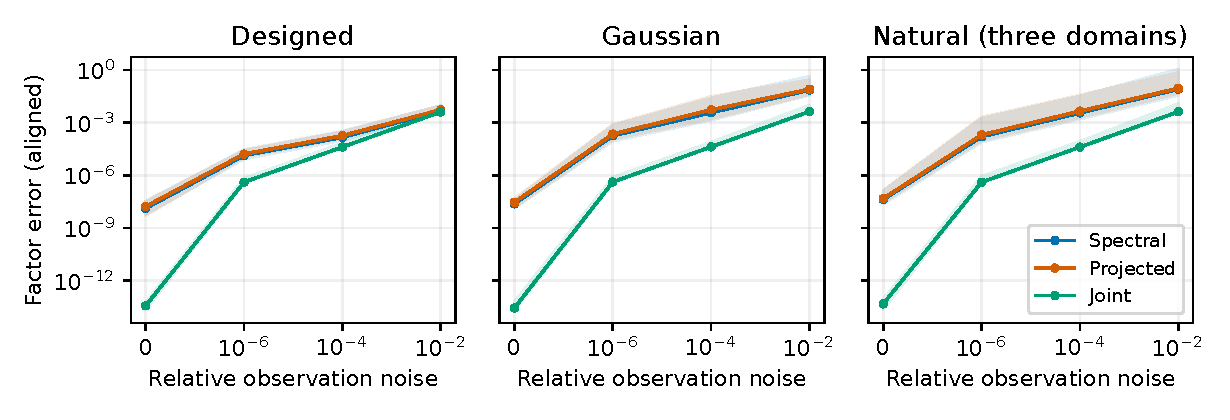
\includegraphics[width=\linewidth]{figures/llm_recovery.pdf}
\caption{Recovery with four queries. Lines show medians and shaded bands
 the 10th--90th percentiles over all 27 checkpoints; the natural panel also
includes all three domains. These are descriptive spreads across correlated
cases, not confidence intervals. Noiseless results use controlled FP64
factor responses, not full-LLM FP64 inference.}
\label{fig:llm-recovery}
\end{figure}

\paragraph{Acceptance rules after calibration.}
Four separate Pythia adapter checkpoints, with general-text validation
queries only, fix acceptance thresholds before held-out recovery scoring.
Defining an error above $0.10$ as bad, the combined joint-fit rule accepted
all 1,080 sufficient-rank cases without accepting a bad output. The
residual-only rule accepted 868, also without a bad output. The absence of
bad outputs in these cases prevents a comparison of the rules' ability to
detect them. For projected spectral recovery,
 the combined rule accepts 43 bad outputs among 1,056, versus 20 among 1,037
for residual-only; its largest accepted error is $6.19$.
Raw spectral recovery has an all-reject calibrated policy under the strict
simplex gate, even though many of its factor errors are small.
Table~\ref{tab:llm-acceptance} retains all denominators. The earlier synthetic
study also retains a combined-rule accepted-bad fraction of $5.16\%$,
above its $5\%$ target. Neither calibration nor candidate-local diagnostics
replace the theorem's externally specified domain assumptions.

\paragraph{Finite precision and decision quality.}
The controlled response formula agrees with autodiff within
$1.62\times10^{-16}$ relative error. Finite-step subtraction is less
reliable: at step $10^{-5}$, FP32 errors range from $0.040$ to $0.102$,
and BF16 errors from $1.00$ to $1.95$. Separately, shrinking the router-rank
margin in learned factors amplifies noisy recovery error by roughly three
orders of magnitude in the registered secondary stress test
(Figure~\ref{fig:llm-conditioning}).

At the nine prespecified checkpoints, balanced coefficient assignment
using recovered routers at noise $10^{-4}$ and $10^{-2}$ reproduced every
native router partition. The fixed balanced Lloyd heuristic applied to
effective parameters produced the same nine partitions. With equal-budget
refitting and 64 recovery updates, coordinate recovery therefore showed
no advantage over this simpler control. Random balanced
 groups worsen general-text NLL after recovery at all nine checkpoints,
while code/math differences have mixed signs. These are token-loss results,
not generation accuracy or realized inference speedups. Detailed action
results, repeated-action numerical controls, costs, and independent CPU
replays are in Appendix~\ref{app:llm-study}.


\subsection{Can real training enter a decision disagreement?}
\label{sec:training-crossings}

The agreement at the original nine checkpoints did not extend to the full
saved set. A post hoc analysis of all 27 checkpoints found seven
coefficient/weight-Lloyd disagreements. Exhaustive enumeration on
Pythia-160M also separates global weight and response optima in two of its
three checkpoints (Appendix~\ref{app:dynamics-experiments}). These observations motivated a separate trajectory experiment. The
original decision test and its fixed evaluation set remain as reported.

\paragraph{Ordinary initialization and natural-language losses.}
We run Pythia-160M, Qwen3-0.6B and SmolLM2-360M with three adapter seeds and
two optimizers, AdamW and momentum-free SGD, for 18 complete 256-step runs.
The loss is ordinary WikiText next-token cross entropy, with no grouping
term or constructed target. Each run trains a $K=4$, 64-channel shared
module on 12 uniformly selected attention output projections; the backbone
is frozen. Restricting the selected depth makes all 15,400 balanced
partitions enumerable at \emph{every} update. This differs from the
all-eligible-layer recovery study. Models, seeds, steps and decision criteria
were fixed before this grid; the grid itself is exploratory, motivated by
previous checkpoint observations.

Table~\ref{tab:training-crossings} reports all runs. Four of nine AdamW
runs entered coefficient/weight disagreement; one changed only the
coefficient partition. All nine entered router-clustering/weight
disagreement, and eight remained in disagreement for at least five
recorded states. None of the nine SGD runs crossed under the same,
unretuned learning-rate schedule. These are dependent finite-run counts, not estimates of a
population frequency or an optimized AdamW--SGD comparison.

\begin{table}[t]
\centering\small
\begin{tabular}{llrrr}
\toprule
Model & Optimizer & Coefficient & Router only & Response \\
\midrule
Pythia-160M & AdamW & 1/3 & 0/3 & 3/3 \\
Qwen3-0.6B & AdamW & 1/3 & 0/3 & 3/3 \\
SmolLM2-360M & AdamW & 2/3 & 1/3 & 3/3 \\
All three & SGD & 0/9 & 0/9 & 0/9 \\
\bottomrule\end{tabular}
\caption{Runs with at least one strict agreement-to-disagreement transition against global weight clustering, over the entire 256-step trajectory. Coefficient means $S_A$ assignment; router only is its subset with unchanged weight partition; response means $J_A$ clustering under the Euclidean-response objective, not an AdamW-optimal decision. All runs use 12 selected projections, $K=4$, and 64 channels. Counts are descriptive, not prevalence estimates.}
\label{tab:training-crossings}
\end{table}


In SmolLM2 seed 1, coefficient and weight partitions agree at update 70.
At update 71, the old-minus-new coefficient score changes from
$2.61\times10^{-5}$ to $-1.66\times10^{-3}$ while the weight partition
stays fixed, with global runner-up gaps $1.84$ and $1.86$.
A fresh pretrained-backbone forward/backward pass and restored AdamW
update reproduce the stored loss, gradients and update exactly in the
same environment. This reproduced a crossing under the natural task loss and AdamW. The
Euclidean-flow theorem concerns a different optimizer.

\paragraph{A controlled local reproduction on the real model.}
We then select that real update-70 state and its next recorded text batch,
fix the batch, and optimize the unchanged next-token loss with equal-rate,
no-momentum, unclipped SGD. No factors or targets are constructed.
The state was selected \emph{post hoc}, so this local experiment is
separate from the ordinary-initialization grid. All four step sizes $0.02,0.01,0.005,0.0025$ cross
while preserving the global weight optimum. A zero-rate FP32 control is unchanged.
FP32 initially obscures refinement through accumulated rounding; an explicit
precision follow-up retains all runs and evaluates the shared injection
and RMS normalization without downcasting. In FP64, adjacent-resolution
endpoint distances are $2.06\times10^{-6}$, $1.03\times10^{-6}$ and
$5.14\times10^{-7}$, showing empirical first-order refinement
(Figure~\ref{fig:dynamics-crossing}). The refinement supports the local crossing mechanism in this real model,
although the trajectories remain numerical approximations. The absence of
crossings in the ordinary-SGD grid is unchanged.

\begin{figure}[t]
\centering
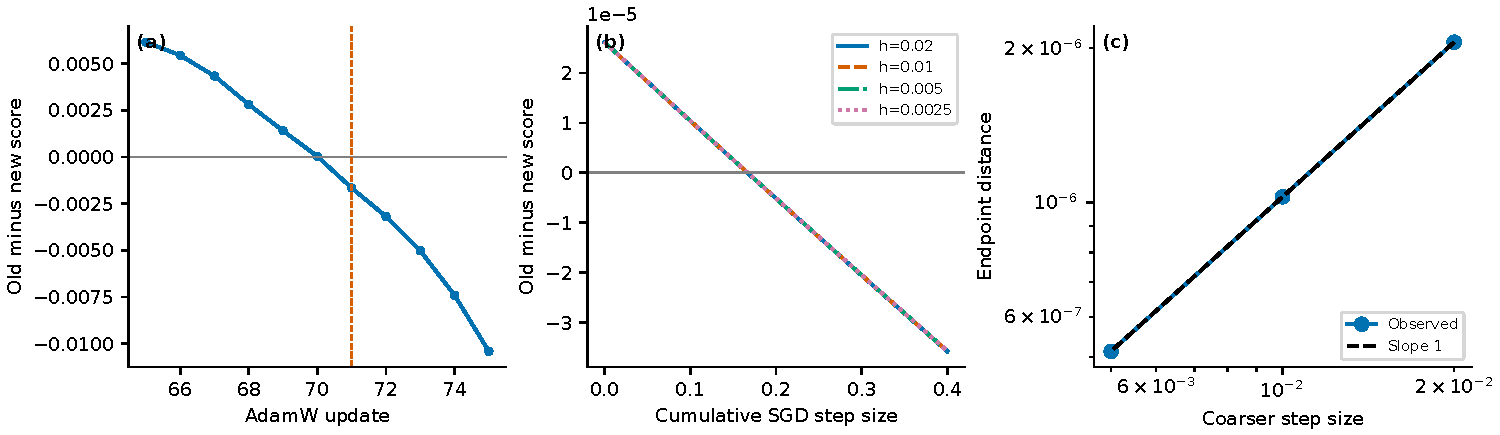
\includegraphics[width=\linewidth]{figures/dynamics_crossing.pdf}
\caption{Complementary real-model evidence. (a) Natural-language AdamW
training of SmolLM2-360M crosses a coefficient boundary at update 71 while
the global weight partition stays fixed. (b) Starting from the selected
real update-70 state, fixed-real-batch FP64 SGD crosses at all four step
sizes, preserving the weight partition. Training time is the sum of step
sizes, not seconds. (c) Adjacent-resolution final parameter distances
approximately halve with step size. These are deterministic trajectory
checks, not confidence intervals or evidence of prevalence.}
\label{fig:dynamics-crossing}
\end{figure}

\paragraph{Discrete optimization of the constructed loss.}
For Theorem~\ref{thm:decision-crossing}, automatic-differentiation SGD
on the fixed squared loss reproduces crossing in all eight step-size/precision
settings, with a zero-gradient control and 60 retained initialization
perturbations. The FP64 endpoint errors against a forward ODE reference
halve with step size. Appendix~\ref{app:dynamics-experiments} records the
noneligible perturbations, numerical precision corrections, all natural-run
outcomes, and exact reproduction settings. Together, the studies show that training can reach disagreement in the
specified shared module. Whether crossings are common, or full factor
recovery improves task performance, remains open.
